\section{從級數到積分}
  \subsection{傅立葉級數}
  根據課本\,11.1\,的內容,因為正弦\,(sine)\,與餘弦\,(cosine)\,函數之間具有正交性\,(orthogonality),任何一個具有週期性的函數\,\(f(x)\)\,均能以傅立葉級數的形式表示:
  \[f(x)=a_0+\sum_{n=1}^{\infty}\left[a_n\cos{\left(\frac{n\pi x}{L}\right)}+b_n\sin{\left(\frac{n\pi x}{L}\right)}\right]\eqno{(1.1)}\]
  其中
  \[a_0=\frac{1}{2L}\int_{-L}^{L}f(v)\,dv\eqno{(1.2)}\]
  \[a_n=\frac{1}{L}\int_{-L}^{L}{f(v)\cos{\left(\frac{n\pi x}{L}\right)}\,dv}\eqno{(1.3)}\]
  \[b_n=\frac{1}{L}\int_{-L}^{L}{f(v)\sin{\left(\frac{n\pi x}{L}\right)}\,dv}\eqno{(1.4)}\]
  且\,\(2L\)\,即為\,\(f(x)\)\,的週期。而為了之後推導上的便利性,我們設
  \[w_n=\frac{n\pi}{L}\quad\text{與}\quad\Delta w=\frac{\pi}{L}\]
  故式\,(1.1)\,可被改寫為
  \[f(x)=a_0+\sum_{n=1}^{\infty}\left[a_n\cos(w_nx)+b_n\sin(w_nx)\right]\eqno{(1.5)}\]
  而將係數\,\(a_0\)、\(a_n\)、\(b_n\)\,代回式\,(1.5)\,並整理的結果為
  \[f(x)=\frac{1}{2L}\int_{-L}^{L}f(v)\,dv
  +\frac{1}{\pi}\sum_{n=1}^{\infty}\left[
    \cos(w_nx)\int_{-L}^{L}{f(v)\cos(w_nv)\,dv}+
    \sin(w_nx)\int_{-L}^{L}{f(v)\sin(w_nv)\,dv}
  \right]\Delta w\eqno{(1.6)}\]

  \subsection{實數域上的傅立葉積分}
  但是傅立葉級數有一個致命性的缺點:因為絕大部分的函數都是非週期性的,它們似乎都不適用於這個數學方法。要解決這個問題,我們必須以另一個角度探討函數的週期性。首先觀察以下的函數圖形:
  \begin{center}
    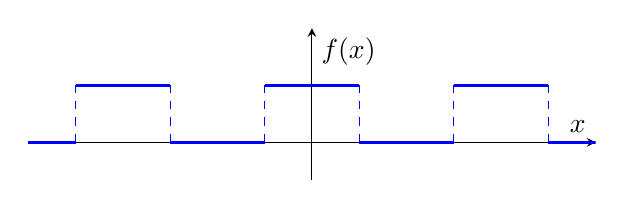
\begin{tikzpicture}
      \begin{axis}[axis lines=middle,
                   ticks=none,
				   xlabel={\(x\)}, ylabel={\(f(x)\)},
				   xmin=-6, xmax=6,ymin=-1, ymax=3,
				   width=250pt, height=100pt]
		\draw[-, very thick, blue](axis cs: -1, 1.5)--(axis cs:  1, 1.5);
        \draw[-, very thick, blue](axis cs: -1, 0  )--(axis cs: -3, 0  );
        \draw[-, very thick, blue](axis cs:  1, 0  )--(axis cs:  3, 0  );
        \draw[-, very thick, blue](axis cs: -3, 1.5)--(axis cs: -5, 1.5);
        \draw[-, very thick, blue](axis cs:  3, 1.5)--(axis cs:  5, 1.5);
        \draw[-, very thick, blue](axis cs:  5, 0  )--(axis cs:  7, 0  );
        \draw[-, very thick, blue](axis cs: -5, 0  )--(axis cs: -7, 0  );

        \draw[-, dashed, blue](axis cs: 5, 0)--(axis cs: 5, 1.5);
        \draw[-, dashed, blue](axis cs: 3, 0)--(axis cs: 3, 1.5);
        \draw[-, dashed, blue](axis cs: 1, 0)--(axis cs: 1, 1.5);
        \draw[-, dashed, blue](axis cs: -5, 0)--(axis cs: -5, 1.5);
        \draw[-, dashed, blue](axis cs: -3, 0)--(axis cs: -3, 1.5);
        \draw[-, dashed, blue](axis cs: -1, 0)--(axis cs: -1, 1.5);
      \end{axis}
    \end{tikzpicture}
  \end{center}
  \noindent 因為圖中存在多個具有相同間距的脈衝波,我們理所當然地會認為該函數具有週期性,但是當我們增加週期\,\(2L\)\,的值,相鄰的兩個脈衝波間距也會增大:
  \begin{center}
    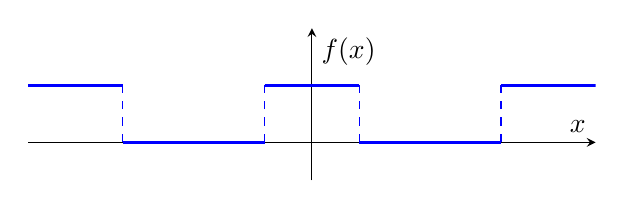
\begin{tikzpicture}
      \begin{axis}[axis lines=middle,
                   ticks=none,
				   xlabel={\(x\)}, ylabel={\(f(x)\)},
				   xmin=-6, xmax=6,ymin=-1, ymax=3,
				   width=250pt, height=100pt]
		\draw[-, very thick, blue](axis cs: -1, 1.5)--(axis cs:  1, 1.5);
        \draw[-, very thick, blue](axis cs: -1, 0  )--(axis cs: -4, 0  );
        \draw[-, very thick, blue](axis cs: -4, 1.5)--(axis cs: -6, 1.5);
        \draw[-, very thick, blue](axis cs:  1, 0  )--(axis cs:  4, 0  );
        \draw[-, very thick, blue](axis cs:  4, 1.5)--(axis cs:  6, 1.5);

        \draw[-, dashed, blue](axis cs: -1, 0)--(axis cs: -1, 1.5);
        \draw[-, dashed, blue](axis cs: -4, 0)--(axis cs: -4, 1.5);
        \draw[-, dashed, blue](axis cs:  1, 0)--(axis cs:  1, 1.5);
        \draw[-, dashed, blue](axis cs:  4, 0)--(axis cs:  4, 1.5);
      \end{axis}
    \end{tikzpicture}
  \end{center}
  \begin{center}
    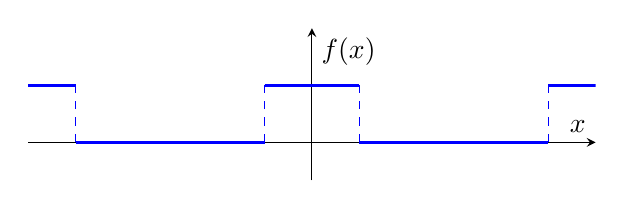
\begin{tikzpicture}
      \begin{axis}[axis lines=middle,
                   ticks=none,
				   xlabel={\(x\)}, ylabel={\(f(x)\)},
				   xmin=-6, xmax=6,ymin=-1, ymax=3,
				   width=250pt, height=100pt]
		\draw[-, very thick, blue](axis cs: -1, 1.5)--(axis cs:  1, 1.5);
        \draw[-, very thick, blue](axis cs: -1, 0  )--(axis cs: -5, 0  );
        \draw[-, very thick, blue](axis cs: -5, 1.5)--(axis cs: -6, 1.5);
        \draw[-, very thick, blue](axis cs:  1, 0  )--(axis cs:  5, 0  );
        \draw[-, very thick, blue](axis cs:  5, 1.5)--(axis cs:  6, 1.5);

        \draw[-, dashed, blue](axis cs: -1, 0)--(axis cs: -1, 1.5);
        \draw[-, dashed, blue](axis cs: -5, 0)--(axis cs: -5, 1.5);
        \draw[-, dashed, blue](axis cs:  1, 0)--(axis cs:  1, 1.5);
        \draw[-, dashed, blue](axis cs:  5, 0)--(axis cs:  5, 1.5);
      \end{axis}
    \end{tikzpicture}
  \end{center}
  \noindent 而當\,\(2L\)\,的值繼續增大,我們就無法在相同的\,\(x\)\,值區間內觀察到其它的波峰:
  \begin{center}
    \begin{tikzpicture}
      \begin{axis}[axis lines=middle,
                   ticks=none,
				   xlabel={\(x\)}, ylabel={\(f(x)\)},
				   xmin=-6, xmax=6,ymin=-1, ymax=3,
				   width=250pt, height=100pt]
		\draw[-, very thick, blue](axis cs: -1, 1.5)--(axis cs:  1, 1.5);
        \draw[-, very thick, blue](axis cs: -1, 0  )--(axis cs: -6, 0  );
        \draw[-, very thick, blue](axis cs:  1, 0  )--(axis cs:  6, 0  );

        \draw[-, dashed, blue](axis cs: -1, 0)--(axis cs: -1, 1.5);
        \draw[-, dashed, blue](axis cs:  1, 0)--(axis cs:  1, 1.5);
      \end{axis}
    \end{tikzpicture}
  \end{center}
  \noindent 雖然畫面上只留下了一個脈衝波,我們仍然不能否認該函數具有週期性的事實,因為其餘的波峰只是超出了畫面。同樣地,當我們定義一個函數不具有週期性時,純粹只是因為它們具有無限大的週期,而無法在有限的範圍下被觀察到。
  \\\\
  當週期\,\(2L\)\,趨近於無限大,也就是\,\(L\)\,趨近於無限大時,式\,(1.6)\,中的
  \[\frac{1}{2L}\quad\text{與}\quad\Delta w=\frac{\pi}{L}\]
  都同樣會趨近於\,\(0\)。因此式\,(1.6)\,中的第一項可以直接消去:
  \[f(x)=\frac{1}{\pi}\sum_{n=1}^{\infty}\left[
    \cos(w_nx)\int_{-L}^{L}{f(v)\cos(w_nv)\,dv}+
    \sin(w_nx)\int_{-L}^{L}{f(v)\sin(w_nv)\,dv}
  \right]\Delta w\eqno{(1.7)}\]
  但是剩餘的級數項並不能直接消去,因為它是一個無限級數。不過根據黎曼積分的定義,這裡的
  \[\sum_{n=1}^{\infty}\left[
    \cos(w_nx)\int_{-L}^{L}{f(v)\cos(w_nv)\,dv}+
    \sin(w_nx)\int_{-L}^{L}{f(v)\sin(w_nv)\,dv}
  \right]\Delta w\]
  即能改寫為積分式
  \[\int_{0}^{\infty}\left[
    \cos(wx)\int_{-L}^{L}{f(v)\cos(wv)\,dv}+
    \sin(wx)\int_{-L}^{L}{f(v)\sin(wv)\,dv}
  \right]dw\]
  因此式\,(1.7)\,又能被改寫為
  \[f(x)=\frac{1}{\pi}\int_{0}^{\infty}\left[
    \cos(wx)\int_{-L}^{L}{f(v)\cos(wv)\,dv}+
    \sin(wx)\int_{-L}^{L}{f(v)\sin(wv)\,dv}
  \right]dw\eqno{(1.8)}\]
  將其稍作整理,我們便能得到傅立葉積分的標準形式:
  \[f(x)=\int_{0}^{\infty}[A(w)\cos(wx)+B(w)\sin(wx)]\,dw\eqno{(1.9)}\]
  其中
  \[A(w)=\frac{1}{\pi}\int_{-\infty}^{\infty}f(v)\cos(wv)\,dv\eqno{(1.10)}\]
  \[B(w)=\frac{1}{\pi}\int_{-\infty}^{\infty}f(v)\sin(wv)\,dv\eqno{(1.11)}\]

  \subsection{複數域上的傅立葉積分}
  我們接著再對式\,(1.9)\,進行分析。代回係數後我們會得到式\,(1.12):
  \[f(x)=\frac{1}{\pi}\int_{0}^{\infty}\left[\cos(wx)\int_{-\infty}^{\infty}f(v)\cos(wv)\,dv+\sin(wx)\int_{-\infty}^{\infty}f(v)\sin(wv)\,dv\right]\,dw\eqno{(1.12)}\]
  接著合併積分項:
  \[f(x)=\frac{1}{\pi}\int_{0}^{\infty}\int_{-\infty}^{\infty}f(v)\left[\cos(wx)\cos(wv)+\sin(wx)\sin(wv)\right]\,dv\,dw\eqno{(1.13)}\]
  而根據三角函數的和差角公式,
  \[\cos(wx)\cos(wv)+\sin(wx)\sin(wv)\]
  即為
  \[\cos(wx-wv)\]
  的展開,故式\,(1.13)\,可以表示為
  \[f(x)=\frac{1}{\pi}\int_{0}^{\infty}\int_{-\infty}^{\infty}f(v)\cos(wx-wv)\,dv\,dw\eqno{(1.14)}\]
  又因為\,\(f(v)\)\,對變數\,\(w\)\,而言為一常數,且\,\(\cos(wx-wv)\)\,為偶函數,上式又可以改寫為
  \[f(x)=\frac{1}{2\pi}\int_{-\infty}^{\infty}\int_{-\infty}^{\infty}f(v)\cos(wx-wv)\,dv\,dw\eqno{(1.15)}\]
  最後因為正弦函數為奇函數,因此將它加入\,(1.15)\,中的積分式後,並不會對整體的結果造成影響:
  \[f(x)=\frac{1}{2\pi}\int_{-\infty}^{\infty}\int_{-\infty}^{\infty}f(v)[\cos(wx-wv)+i\sin(wx-wv)]\,dv\,dw\eqno{(1.16)}\]
  因此根據歐拉公式\,(Euler's formula)
  \[e^{ix}=\cos x+i\sin x\eqno{(1.17)}\]
  我們可以得出複數域上的傅立葉積分
  \[f(x)=\frac{1}{2\pi}\int_{-\infty}^{\infty}\int_{-\infty}^{\infty}f(v)\exp{[iw(x-v)]}\,dv\,dw\eqno{(1.18)}\]
  並定義
  \[\hat{f}(w)
  =\mathfrak{F}\left[f(x)\right]
  =\frac{1}{\sqrt{2\pi}}\int_{-\infty}^{\infty}f(x)\exp{(-iwx)}\,dx\eqno{(1.19)}\]
  與
  \[f(x)
  =\mathfrak{F}^{-1}\left[\hat{f}(x)\right]
  =\frac{1}{\sqrt{2\pi}}\int_{-\infty}^{\infty}\hat{f}(w)\exp{(iwx)}\,dw\eqno{(1.20)}\]
  其中\,\(\mathfrak{F}\)\,與\,\(\mathfrak{F}^{-1}\)\,分別代表傅立葉轉換\,(Fourier transform, FT)\,與逆傅立葉轉換\,(Inverse Fourier transform, IFT)。
